% Cosine similarity distribution for Tier 2 semantic circulus detection
% Data: 3,919 Tier-1-negative definitions, E5-large embeddings
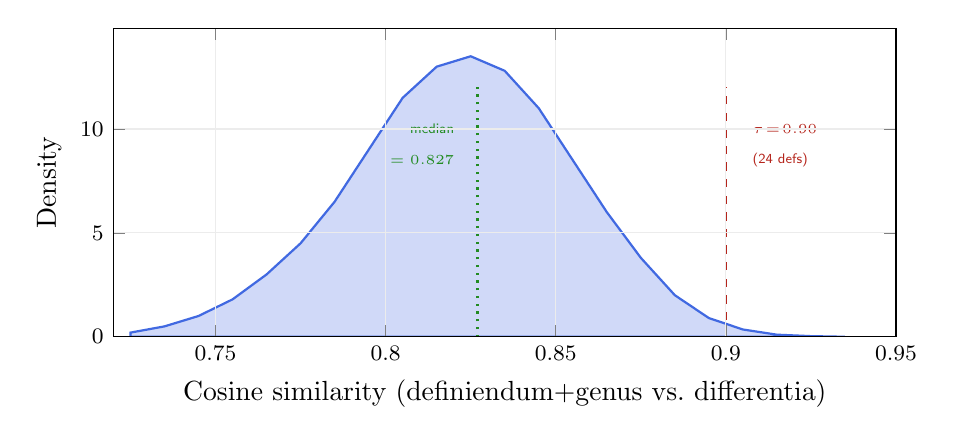
\begin{tikzpicture}
\begin{axis}[
  width=0.95\linewidth,
  height=5.5cm,
  xlabel={Cosine similarity (definiendum+genus vs.\ differentia)},
  ylabel={Density},
  xmin=0.72, xmax=0.95,
  ymin=0,
  xtick={0.75, 0.80, 0.85, 0.90, 0.95},
  xticklabel style={font=\footnotesize},
  yticklabel style={font=\footnotesize},
  grid=major,
  grid style={gray!15},
  area style,
  no markers,
]

% Approximate density from histogram bins
\addplot[fill=RoyalBlue!25, draw=RoyalBlue, thick] coordinates {
  (0.725, 0.2) (0.735, 0.5) (0.745, 1.0) (0.755, 1.8) (0.765, 3.0)
  (0.775, 4.5) (0.785, 6.5) (0.795, 9.0) (0.805, 11.5) (0.815, 13.0)
  (0.825, 13.5) (0.835, 12.8) (0.845, 11.0) (0.855, 8.5) (0.865, 6.0)
  (0.875, 3.8) (0.885, 2.0) (0.895, 0.9) (0.905, 0.35) (0.915, 0.10)
  (0.925, 0.03) (0.935, 0.0)
} \closedcycle;

% Threshold line at 0.90
\draw[BrickRed, thick, dashed] (axis cs:0.90,0) -- (axis cs:0.90,12);
\node[font=\tiny\sffamily, text=BrickRed, anchor=west] at (axis cs:0.905,10) {$\tau\!=\!0.90$};
\node[font=\tiny\sffamily, text=BrickRed, anchor=west] at (axis cs:0.905,8.5) {(24 defs)};

% Median line
\draw[ForestGreen, thick, dotted] (axis cs:0.827,0) -- (axis cs:0.827,12);
\node[font=\tiny\sffamily, text=ForestGreen, anchor=east] at (axis cs:0.823,10) {median};
\node[font=\tiny\sffamily, text=ForestGreen, anchor=east] at (axis cs:0.823,8.5) {$= 0.827$};

\end{axis}
\end{tikzpicture}
